\section{Simulations}
\label{sec:sims}

We characterize the method in a synthetic model that matches the observation model of Section~\ref{sec:setting} in the vantablack setting, which is the setting of the real data in Section~\ref{sec:realdata}: agents respond to few, self-selected, unpaired queries, and the queries themselves are estimated from context and therefore observed with error. The black box setting ($\sigma_q=0$) appears only as a reference level. The two problems of Section~\ref{sec:problem} are evaluated in two separate experiments, each with its own design and its own error criteria: detection (P0, Section~\ref{sec:exp-detect}) and membership estimation (P1, Section~\ref{sec:exp-member}). Code and the full grid specification are in the supplement.

\todo{All grids are to be run on larger infrastructure ($R=200$ replicates per cell, $B=200$ permutations). The figures currently in the draft are rendered from a local pilot of the base configuration and are placeholders; every ``Results'' paragraph below is to be written from the full run.}

\subsection{Generative model}
\label{sec:sim-model}

Agent $i$ has a latent position $a_i\sim N(0,I_3)$. The query space has $K=6$ topic centers $\mu_k\sim 1.5\,N(0,I_6)$, and agent $i$ has topic preferences $\pi_i\sim\mathrm{Dir}(\alpha\mathbf 1_K)$; small $\alpha$ concentrates each agent on few topics, so that different agents respond to different queries. At each time point agent $i$ responds to $m_i\sim 2+\mathrm{Poisson}(m-2)$ queries, each drawn by sampling a topic from $\pi_i$ and a query $u=\mu_k+0.5\,\xi$, $\xi\sim N(0,I_6)$. The embedded response is
\begin{equation}
x \;=\; B a_i + W u + \varepsilon, \qquad \varepsilon\sim N(0,\sigma_x^2 I_{12}),
\end{equation}
with $B\in\R^{12\times 3}$ having orthonormal columns, $W = 0.5\cdot G/\sqrt 6$ for a Gaussian matrix $G$, and $\sigma_x=0.5$. The response therefore depends on the agent through $Ba_i$, on the query through $Wu$, and on noise. After burn-in, $a_i\to a_i+\delta v$ for $i\in S$, with $v$ a random unit vector; because $B$ has orthonormal columns, $\delta$ is also the mean shift in response space, in units of twice the per-coordinate noise. Optionally all agents share a common drift $c\sim N(0,\sigma_c^2 I_3)$. The observed query is the estimate $\hat u = u+\sigma_q\zeta$, $\zeta\sim N(0,I_6)$, with $\sigma_q=1$ by default, which is comparable to the within-topic spread and about a quarter of the separation between topics; $\sigma_q=0$ recovers the black box setting. The base configuration is $N=50$, $|S|=5$, $m=10$, $\sigma_q=1$, $\alpha=1$, $\sigma_c=0$.

\subsection{Method as run}
\label{sec:sim-method}

The query kernel is Gaussian with bandwidth set by the median heuristic on the observed queries; the response kernel is linear, so that the induced distance between two units is a query-weighted mean-shift distance. Self-affinities exclude the $j=l$ terms: without this, $\hat A_{aa}$ carries the response noise variance $\sigma_x^2 p_\X$ with weight equal to the diagonal share of the query-kernel mass, and every within-agent distance $\hat D^2_{(i,t_0),(i,t)}$ is biased upward by an amount comparable to $\delta^2$; the U-statistic form removes the bias and requires only $m_i\ge 2$. Units are embedded jointly in $d=3$ dimensions, displacements are centered by the coordinate-wise median and whitened by a 25\%-trimmed covariance, and the candidate family consists of $k$-means clusters for $k\in\{2,3,4\}$ and nested top-$r$ sets along the leading direction. The scan statistic is the maximum of the size-standardized $T(S)$, with per-size null moments from one set of permutations and the null distribution of the maximum from an independent set; using the same permutations for both inflated the Type~I error in pilot runs. Each permutation reassigns every agent's (query, response) pairs across the two time points preserving counts; only the assignment matrix $Z$ in \eqref{eq:matrix} changes.

\subsection{Experiment 1: detection}
\label{sec:exp-detect}

\paragraph{Question.} Does the test reject when a colluding subnetwork is present, and not otherwise, and how does this depend on the factors that \eqref{eq:conc} says it should?

\paragraph{Design.} Starting from the base configuration we vary one factor at a time, each crossed with $\delta\in\{0,0.5,1,1.5\}$: the effect size alone over the finer grid $\delta\in\{0,0.25,\dots,2\}$; the number of agents $N\in\{20,50,100,200\}$ with $|S|=5$ fixed, so that the subnetwork is a shrinking minority; the responses per agent per time point $m\in\{3,5,10,20,40\}$; the subnetwork size $|S|\in\{2,3,5,10,15\}$; the query estimation noise $\sigma_q\in\{0,0.5,1,2,4\}$, from the black box reference through the base to a level at which the estimated query is nearly uninformative ($\sigma_q=4$ against a topic separation of about $3.7$); the topic concentration $\alpha\in\{0.1,0.2,1,5\}$, from almost fully unpaired to almost fully paired; and the common drift $\sigma_c\in\{0,0.5,1\}$, a nuisance that median centering is meant to remove. This is $80$ cells.

\paragraph{Error criteria.} \emph{Type~I error}: the rejection rate at level $\alpha=0.05$ over all cells with $\delta=0$, pooled and per cell, so that the level is checked under the nuisances (drift, unpairedness, query noise) and not only under the clean null. \emph{Power}: the rejection rate for $\delta>0$. \emph{Correct detection}: the rate at which the test rejects \emph{and} the returned set overlaps the truth, $\mathrm{Jaccard}(\hat S,S)\ge 0.5$. A scan can reject on a spurious set that has nothing to do with $S$; the gap between power and correct detection is a diagnostic of the candidate family, and correct detection is the quantity an operator cares about.

\begin{figure*}[t]
  \centering
  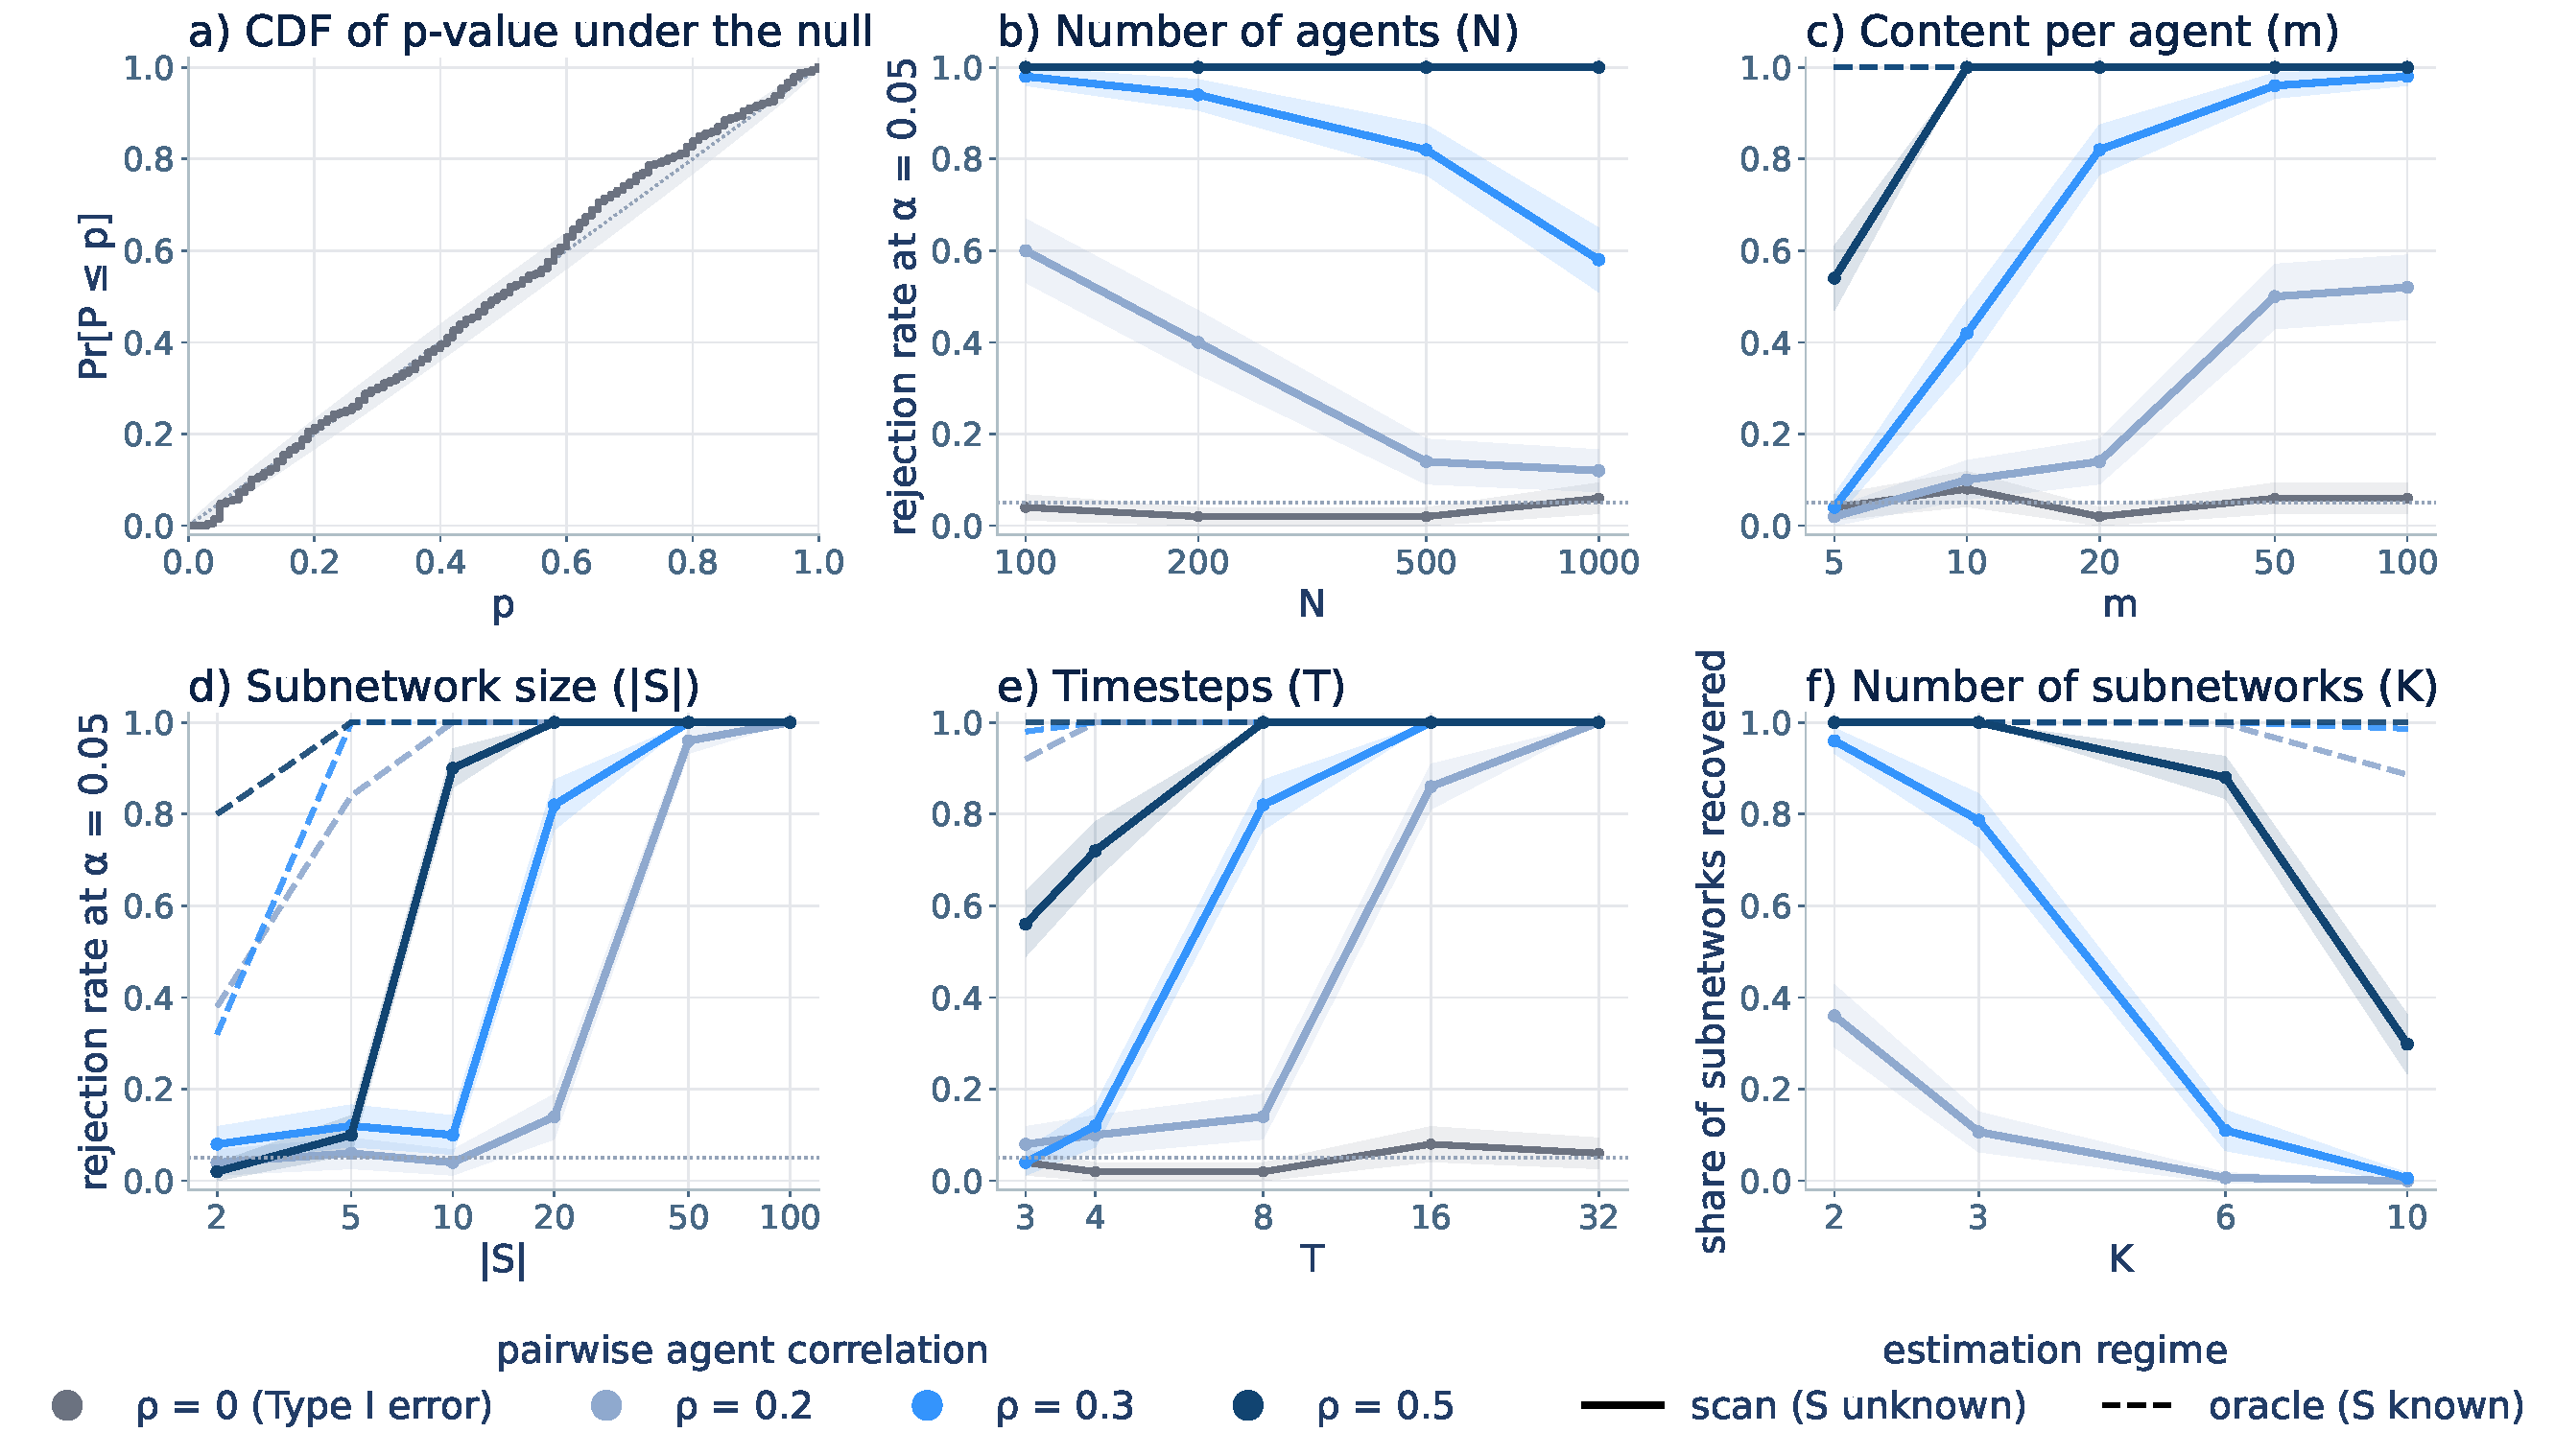
\includegraphics[width=\textwidth]{figures/sim_detection.pdf}
  \caption{Experiment 1 (detection). (a) Rejection rate and correct-detection rate versus $\delta$ in the base configuration, with one standard error. (b) Rejection rate by responses per agent $m$. (c) Rejection rate by query estimation noise $\sigma_q$; $\sigma_q=0$ is the black box reference and $\sigma_q=1$ the base. (d) Type~I error at level $0.05$ by null cell. The remaining factors ($N$, $|S|$, $\alpha$, drift) are in Figure~\ref{fig:sim-detect-app}. \todo{pilot rendering}}
  \label{fig:sim-detect}
\end{figure*}

\paragraph{Results.} \todo{Type~I error pooled over the $\delta=0$ cells and per cell; where the power curve leaves the level and reaches $0.9$ in the base configuration; the $m^{-1/2}$ scaling predicted by \eqref{eq:conc}, i.e.\ whether doubling $m$ shifts the curve by $\sqrt 2$ in $\delta$; the slow decrease in $N$ with $|S|$ fixed; the linear gain in $|S|$ and any loss at $|S|=15$ where the minority assumption behind median centering weakens; the loss from the black box reference $\sigma_q=0$ to the base $\sigma_q=1$ and on to $\sigma_q=4$, which is the cost of the vantablack setting; the price of unpairedness, the factor $\kappa^{-2}$ in \eqref{eq:conc}; and whether drift leaves the level intact. Pilot: Type~I $0.067$ on $60$ null replicates; at $\delta=2$ every smoke-test replicate rejected.}

\subsection{Experiment 2: membership estimation}
\label{sec:exp-member}

\paragraph{Question.} Given that something is present, how much of the colluding subnetwork does the estimate $\hat S$ recover, and how does the answer depend on the subnetwork's size, on competing structure, and on scale?

\paragraph{Design.} Four sub-designs: the subnetwork size $|S|\in\{3,5,10,15\}$ crossed with $\delta\in\{0.5,1,1.5,2,3\}$; two colluding subnetworks, $S$ and a second $S_2$ of size $|S_2|\in\{3,5\}$ moving in an orthogonal direction, crossed with $\delta\in\{1,1.5,2\}$, to test whether the scan returns one of them cleanly or their union; scale with the subnetwork a fixed tenth of the system, $(N,|S|)\in\{(50,5),(100,10),(200,20)\}$, crossed with $\delta\in\{1,1.5,2\}$; and responses per agent $m\in\{5,20,40\}$ at $\delta\in\{1,1.5\}$.

\paragraph{Error criteria.} All reported \emph{unconditionally}: an unrejected replicate still returns the maximizing set, so that a detector with no power cannot look good on membership; conditional-on-rejection versions are in Appendix~\ref{app:sims}. \emph{Jaccard index} $|\hat S\cap S|/|\hat S\cup S|$ is the headline. \emph{Precision} and \emph{recall} are reported separately because their errors have different costs under mitigation: a false inclusion quarantines an innocent agent, a miss leaves a colluder in place. \emph{Nomination AUC} separates ranking quality from the choice of threshold implicit in $\hat S$: agents are ordered by the projection of their centered, whitened displacement onto the direction of $\bar\Delta_{\hat S}$, and the AUC of this ranking against membership in $S$ is reported; this is the vertex-nomination criterion of Section~\ref{sec:related} without seeds. In the two-subnetwork design we report Jaccard against $S$ and against $S_2$ separately.

\begin{figure*}[t]
  \centering
  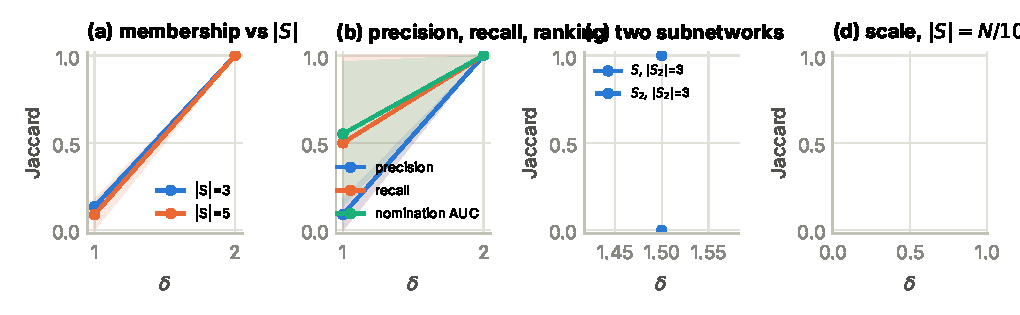
\includegraphics[width=\textwidth]{figures/sim_membership.pdf}
  \caption{Experiment 2 (membership). (a) Jaccard versus $\delta$ by $|S|$. (b) Precision, recall, and nomination AUC in the base configuration. (c) Two colluding subnetworks: Jaccard of $\hat S$ against $S$ (solid) and against $S_2$ (dashed). (d) Scale with $|S|=N/10$. \todo{to be rendered from the full run}}
  \label{fig:sim-member}
\end{figure*}

\paragraph{Results.} \todo{Whether Jaccard tracks correct detection or lags it (the nested-set family tends to return a superset or subset of $S$, which shows as precision below recall or the reverse); whether nomination AUC approaches one before Jaccard does, which would indicate that the ranking is right and the threshold is the limitation; whether with two subnetworks the scan returns the larger one cleanly, the union, or alternates; and whether membership recovery at fixed $|S|/N$ improves or degrades with $N$.}
